\documentclass[12pt]{article}
\usepackage{amsmath,amssymb}
\setlength{\oddsidemargin}{0in}
\setlength{\evensidemargin}{0in}
\setlength{\textheight}{9in}
\setlength{\textwidth}{6.5in}
\setlength{\topmargin}{-0.5in}
\usepackage{enumitem}
\usepackage[table]{xcolor}
\usepackage{graphicx}
\usepackage{listings}
\usepackage{float}
\usepackage{caption}
\usepackage{subcaption}
\usepackage{pdfpages}
\newcommand{\Adv}{{\mathbf{Adv}}}       
\newcommand{\prp}{{\mathrm{prp}}}             
\newcommand{\calK}{{\cal K}}
\newcommand{\outputs}{{\Rightarrow}}                



% Use \textbf{Solution:}\\ to begin your solution.

%%%%%%%%%%%%%%%%%%%%%%%%%%%%%%%%%%%%%%%%%%%%%%%%%%%%%%%%%%%%%%%%%%%%%%%%%%%
\title{\bf Math 151A: Problem Set 7}
\date{ 6/9/2023}
\author{\bf Owen Jones}

\begin{document}
\maketitle


{\small \textbf{Instructions}:
\begin{itemize}
\item Due on Friday, June 9th by 11:59pm.
\item Late HW will not be accepted.
\item Write down all of the details and attach your code to the end of the assignment for full credit (as a PDF).  
\item If you LaTeX your solutions, you will get $5\%$ extra credit. 
\item (T) are ``pencil-and-paper'' problems and (C) means that the problem includes a computational/programming component. 
\end{itemize}}

%Add \newpage  between problems if you are using this to LaTex your solutions
\vspace{1em}

%%%%%%%%%%%%%%%%%%%%%%%%%%%%%%%%%%%%%%%%%%%%%%%%%%%%%%%%
\begin{enumerate}[label=\bfseries Problem \arabic*:]






 
%%%%%%%%%%%%%%%%%%%%%%%%%%%%%%%%%%%%%%%%%%%%%
%%%%%%%%%%%%%%%%%%%%%%%


\item \textbf{(T) Power Method}\\
Use the power method to approximate a dominant eigenvector and eigenvalue of the matrix $A$:

$$A =  \begin{bmatrix}
3 & 0 & 0\\
1 & -1 & 0\\
0& 2 & 8\\
\end{bmatrix},$$

by computing (either by-hand or using a code) $\vec{v}^{(5)}$ and $\lambda^{(5)}=r\left(\vec{v}^{(5)}\right)$ starting with 
$$\vec{v}^{(0)} =  \begin{bmatrix}
1\\
1\\
1
\end{bmatrix}.$$
\vspace{1em}
\textbf{Solution:}\\
$\vec{w}^{(1)}=A\cdot \vec{v}^{(0)}=\begin{bmatrix}
3\\
0\\
10   
\end{bmatrix}$, 
$\vec{v}^{(1)}=\frac{\vec{w}^{(1)}}{||\vec{w}^{(1)}||}=\begin{bmatrix}
\frac{3}{\sqrt{109}}\\
0\\
\frac{10}{\sqrt{109}}
\end{bmatrix}$\\
$\vec{w}^{(2)}=A\cdot \vec{v}^{(1)}=\begin{bmatrix}
\frac{9}{\sqrt{109}}\\
\frac{3}{\sqrt{109}}\\
\frac{80}{\sqrt{109}} 
\end{bmatrix}$, 
$\vec{v}^{(2)}=\frac{\vec{w}^{(2)}}{||\vec{w}^{(2)}||}=\begin{bmatrix}
\frac{9}{\sqrt{6490}}\\
\frac{3}{\sqrt{6490}}\\
\frac{8\sqrt{10}}{\sqrt{649}}
\end{bmatrix}$\\
$\vec{w}^{(3)}=A\cdot \vec{v}^{(2)}=\begin{bmatrix}
\frac{27}{\sqrt{6490}}\\
\frac{3\sqrt{2}}{\sqrt{3245}}\\
\frac{323\sqrt{2}}{\sqrt{3245}} 
\end{bmatrix}$, 
$\vec{v}^{(3)}=\frac{\vec{w}^{(3)}}{||\vec{w}^{(3)}||}=\begin{bmatrix}
\frac{27}{\sqrt{418081}}\\
\frac{6}{\sqrt{418081}}\\
\frac{38\sqrt{17}}{\sqrt{24593}}
\end{bmatrix}$\\
$\vec{w}^{(4)}=A\cdot \vec{v}^{(3)}=\begin{bmatrix}
\frac{81}{\sqrt{418081}}\\
\frac{21}{\sqrt{418081}}\\
\frac{5180}{\sqrt{418081}} 
\end{bmatrix}$, 
$\vec{v}^{(4)}=\frac{\vec{w}^{(4)}}{||\vec{w}^{(4)}||}=\begin{bmatrix}
\frac{81}{\sqrt{26839402}}\\
\frac{21}{\sqrt{26839402}}\\
\frac{2590\sqrt{2}}{\sqrt{13419701}}
\end{bmatrix}$\\
$\vec{w}^{(5)}=A\cdot \vec{v}^{(4)}=\begin{bmatrix}
\frac{243}{\sqrt{26839402}}\\
\frac{30\sqrt{2}}{\sqrt{13419701}}\\
\frac{20741\sqrt{2}}{\sqrt{13419701}} 
\end{bmatrix}$, 
$\vec{v}^{(5)}=\frac{\vec{w}^{(5)}}{||\vec{w}^{(5)}||}=\begin{bmatrix}
\frac{243}{\sqrt{1720818973}}\\
\frac{60}{\sqrt{1720818973}}\\
\frac{41482}{\sqrt{1720818973}}
\end{bmatrix}$\\
$\lambda^{(5)}=r(\vec{v}^{(5)})=(\vec{v}^{(5)})^TA\vec{v}^{(5)}=\frac{13771216559}{1720818973}\approx8.0027$\\
\newpage
 %%%%%%%%%%%%%%%%%%%%%%%%%%%%%%%%%%%
\item \textbf{(T) Power Method}
\begin{itemize}
\item[(a)] Find the eigenvalues and the corresponding eigenvectors of the matrix $A$:

$$A =  \begin{bmatrix}
3 & -1\\
2 & 4
\end{bmatrix}.$$

\item[(b)] Calculate two iterations of the power method starting with 
$$\vec{v}^{(0)} =  \begin{bmatrix}
1\\
1
\end{bmatrix}.$$
\item[(c)] Explain why the power method does not seem to converge to a dominant eigenvector for this problem.
\end{itemize}


\vspace{1em}
\textbf{Solution:}\\
\begin{itemize}
    \item [(a)] $\det(A-\lambda\cdot I)=\lambda^2-7\lambda+14\Rightarrow\lambda=\frac{7}{2}\pm i\frac{\sqrt{7}}{2}$\\
    $(A-\lambda\cdot I)x=0\Rightarrow
    \begin{bmatrix}
    (-\frac{1}{2}-i\frac{\sqrt{7}}{2})x_1-x_2\\
    2x_1+(\frac{1}{2}-i\frac{\sqrt{7}}{2})x_2
    \end{bmatrix}
    =
    \begin{bmatrix}
    0\\
    0
    \end{bmatrix}$
    and 
    $\begin{bmatrix}
    (-\frac{1}{2}+i\frac{\sqrt{7}}{2})x_1-x_2\\
    2x_1+(\frac{1}{2}+i\frac{\sqrt{7}}{2})x_2
    \end{bmatrix}
    =
    \begin{bmatrix}
    0\\
    0
    \end{bmatrix}$\\
    , so $\vec{v}_1=
    \begin{bmatrix}
    -1+\sqrt{7}i\\
    4
    \end{bmatrix}$
    with $\lambda=\frac{7}{2}+i\frac{\sqrt{7}}{2}$
    and $\vec{v}_2=
    \begin{bmatrix}
    -1-\sqrt{7}i\\
    4
    \end{bmatrix}$
    with $\lambda=\frac{7}{2}-i\frac{\sqrt{7}}{2}$
    \item [(b)] 
    $\vec{w}^{(1)}=A\cdot \vec{v}^{(0)}=\begin{bmatrix}
    2\\
    6   
    \end{bmatrix}$, 
    $\vec{v}^{(1)}=\frac{\vec{w}^{(1)}}{||\vec{w}^{(1)}||}=\begin{bmatrix}
    \frac{1}{\sqrt{10}}\\
    \frac{3}{\sqrt{10}}
    \end{bmatrix}$\\
    $\vec{w}^{(2)}=A\cdot \vec{v}^{(1)}=\begin{bmatrix}
    0
    \frac{7\sqrt{2}}{\sqrt{5}}
    \end{bmatrix}$, 
    $\vec{v}^{(2)}=\frac{\vec{w}^{(2)}}{||\vec{w}^{(2)}||}=\begin{bmatrix}
    0\\
    1
    \end{bmatrix}$\\
    $\lambda^{(2)}=r(\vec{v}^{(2)})=(\vec{v}^{(2)})^TA\vec{v}^{(2)}=4$\\
    \item [(c)] Both of the eigenvalues and the eigenvectors of matrix A are complex, so the power method will not converge to a dominant eigenvalue.
\end{itemize}
    \newpage
%%%%%%%%%%%%%%%%%%%%%%%%%%%%%%
 \item \textbf{(C) Classification}\\
Complete the template code on linear algebra and deep learning. Apply your completed code to the dataset provided online. 

\vspace{1em}
\textbf{Solution:}
\begin{figure}[H]
\begin{subfigure}[t!]{.33\textwidth}
   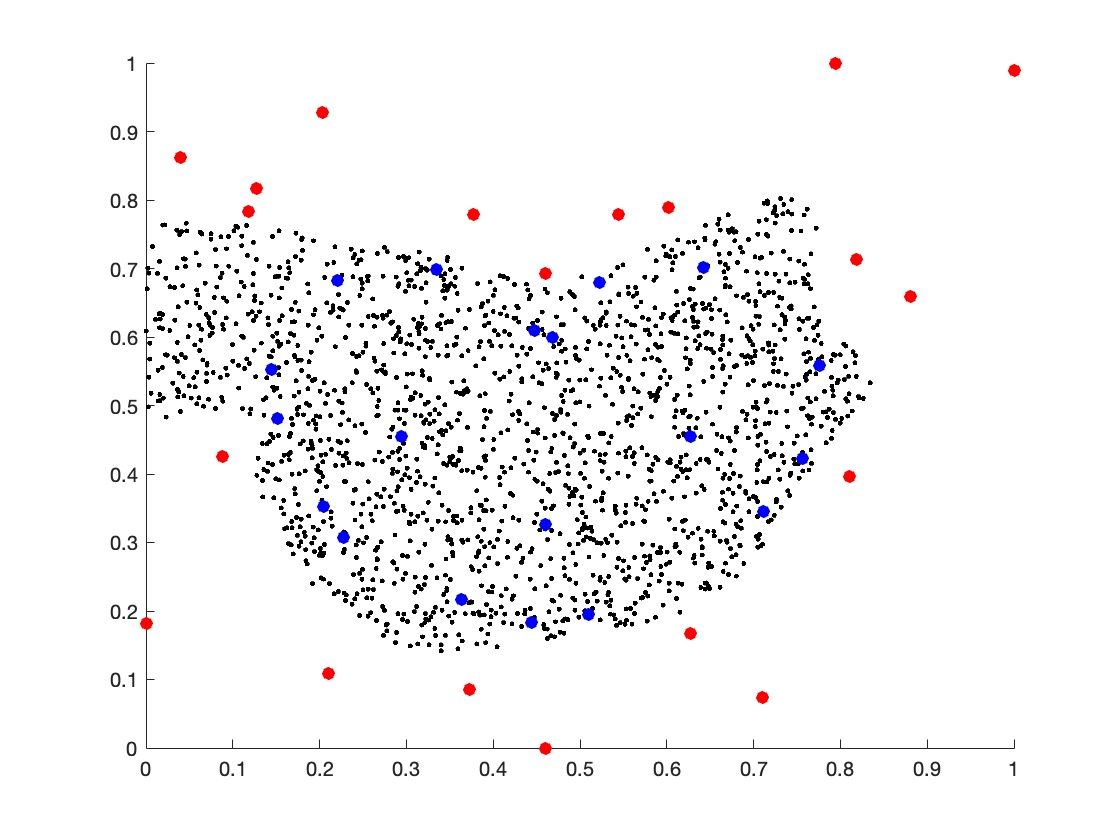
\includegraphics[width=\linewidth]{PS_7_graph_cost.jpg}
\end{subfigure}%
\begin{subfigure}[t!]{.33\textwidth}
  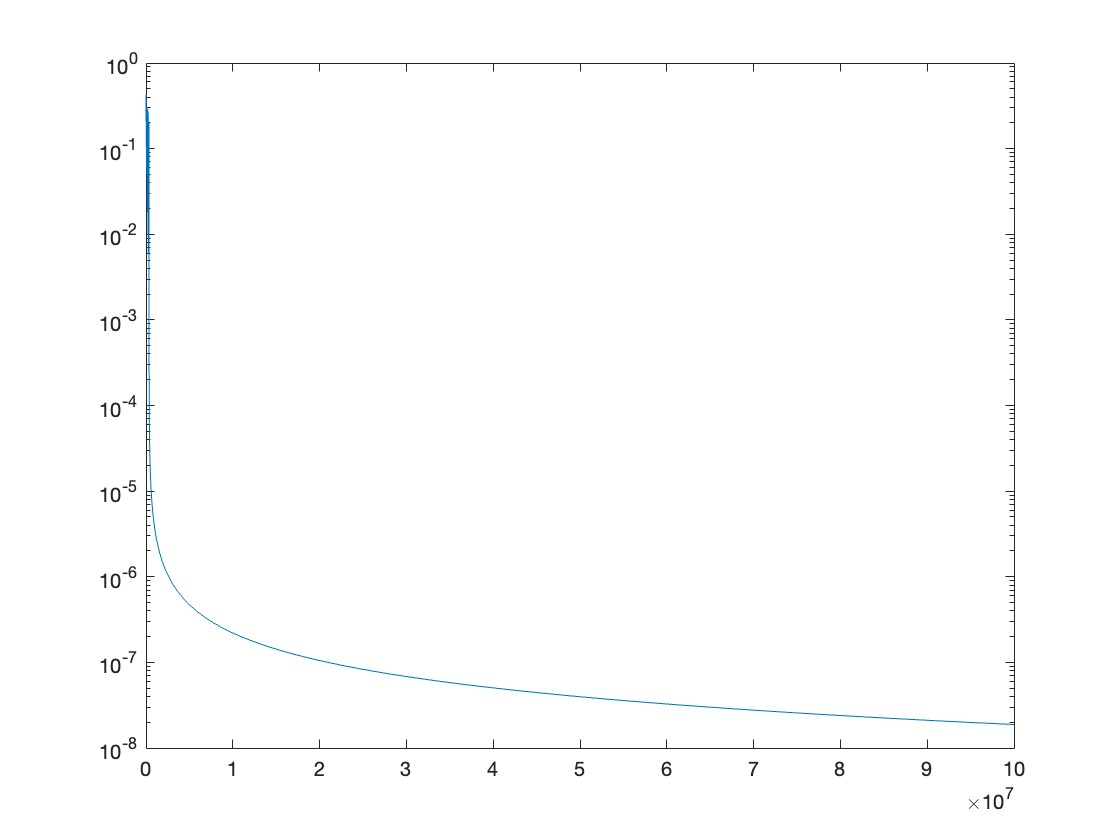
\includegraphics[width=\linewidth]{PS_7_graph_cost_v_time.jpg}
\end{subfigure}%
\begin{subfigure}[t!]{.33\textwidth}
    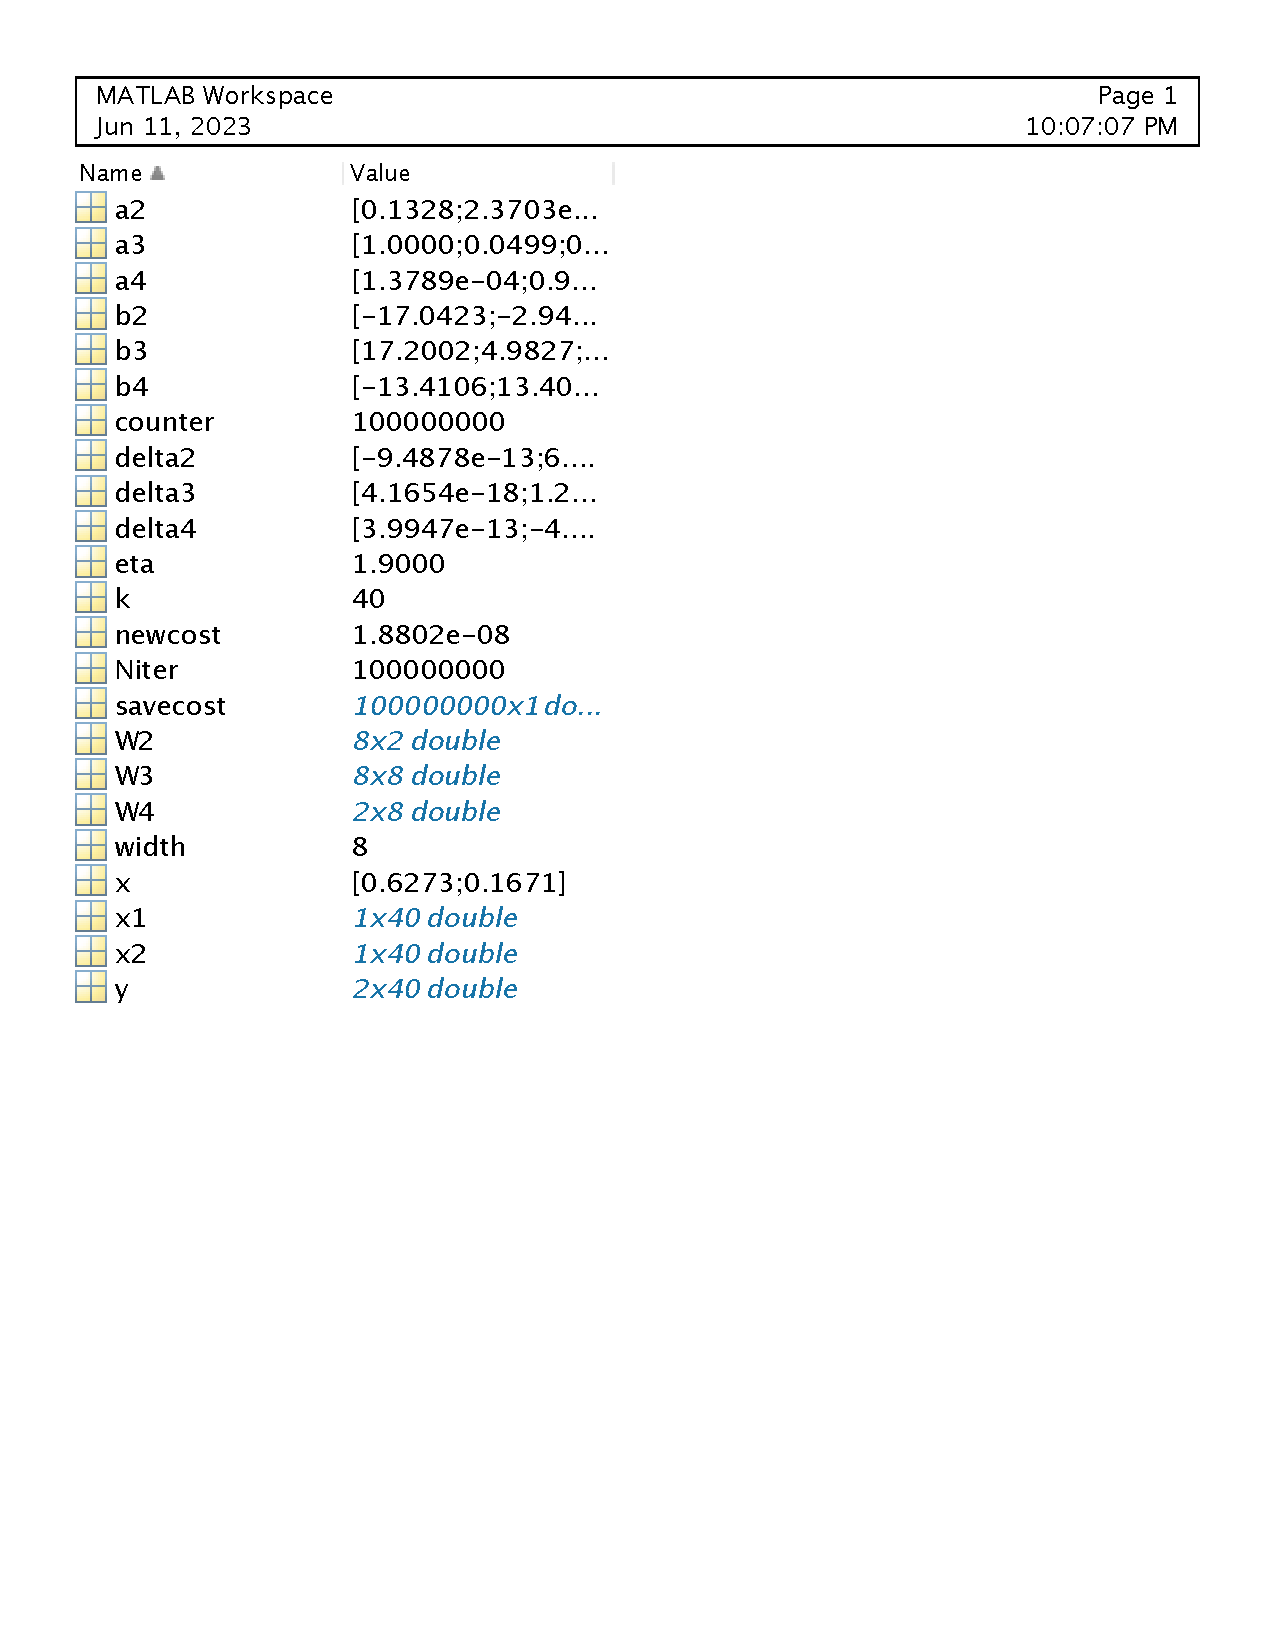
\includegraphics[width=\linewidth]{PS_7_workspace_new.pdf}
  \end{subfigure}%
\end{figure}
%%%%%%%%%%%%%%%%%%%%%%%%%%%%%%%%%%%

\end{enumerate}

\end{document}


